% Chapter discussion

\chapter{Introduction} %-5/10pagine} % Main chapter title

\label{Chapter2} % For referencing the chapter elsewhere, use \ref{Chapter4} 

%----------------------------------------------------------------------------------------

%1. Sequenziamento (mezza pagina)
%2. Modelli: genomica e pangenomica, facendo riferimento al problema reference based.
%3. come si codifica l'informazione: pangenoma (GFA) + bubble e vcf.
%4. HLA e polimorfico, complesso con modelli genomici 


%Grandezza genomi, genomi complessi, definizione pangenoma.


\section{DNA sequencing}
%TODO:
%1.Figura nanopore 
%2.referenze 
%3.  \url{https://ib.bioninja.com.au/standard-level/topic-3-genetics/32-chromosomes/genome-size.html}, aggiungere questo concetto, complessità degli organismi in giga, trovare articolo.


%PER ENZA \url{https://aulascienze.scuola.zanichelli.it/come-te-lo-spiego/2018/04/18/dal-metodo-sanger-a-oggi-40-anni-di-sequenziamento-del-dna/} mi sono ispirata a questi


The process of sequencing determines the exact order of the monomers in a biomolecule, the nucleotides in the case of DNA sequencing. Sequence analyses has many applications, e.g. identify mutations or establish phylogenetic relationships among species. Sanger's method marked the beginning of genomics research and has been successfully until a decade ago when \textit{next generation sequencing (NGS)} was introduced to overcome the main limit of the Sanger sequencing,(\cite{Sanger5463}) i.e. the sequencing volume.

The main feature of NGS sequencing is the high-throughput. Unlike the traditional Sanger method, the NGS allows to analyze many sequences in parallel, reducing analysis times and costs. This reduction has improved over time: the sequencing of the first human genome, based on the Sanger method, required an investment of almost 100M dollars in about ten years, while today the sequence of a human genome can be obtained for less than 1k dollars in one day (\cite{sequencing}). Nevertheless, NGS has limitations too. The main limitation is the initial amplification of DNA sequences, which can introduce random errors in the sequence and leads to the loss of "accessory" information, such as the constellation of epigenetic modifications that are important for understanding the function of a fragment of genome. (\cite{sequencing}) A second important limitations the size of the sequenced regions that covers at its best 700kb making impossible to map large structural variants.

To overcome these limitations, research is now pointing towards \textit{third generation} methods that are oriented toward sequencing very long regions (ideally whole chromosomes) without  prior amplification. Among these methods, nanopore sequencing derives from an observation from the 1980s that when a single-stranded DNA passes through a very narrow channel (nanopore) (Fig:\ref{fig:nanopore.png})generates a flow of ions with a characteristic pattern, which depends uniquely on its sequence. This technology allows sequencing millions of nucleotides without prior amplification of DNA fragments. (\cite{wiki:nanopore}).

\begin{figure}[H]
\centering
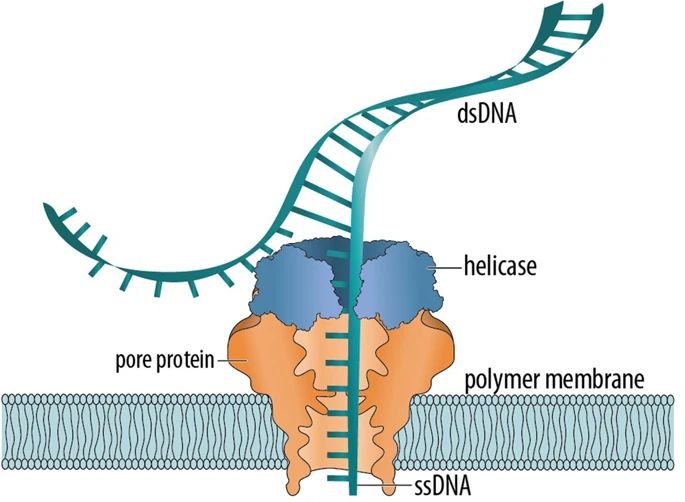
\includegraphics[width=0.70\textwidth]{fig/nanopore.png}
\decoRule
\caption{Schematic representation of a DNA molecule translocating a protein nanopore. The double-stranded DNA (dsDNA) is split by a helicase enzyme, allowing only a single strand (ssDNA) to pass while slowing it enough to achieve sufficient resolution for sequencing" \textit{Adapted from} \cite{sutton2019radiation}"} 
\label{fig:nanopore.png}
\end{figure}







\section{Genome \textit{versus} pangenome}
%TODO: REFERENCE BIAS chiedere ad Erik
%Genomics studies are based on two models: standard and alternative models. 

Standard approaches in sequence analysis relate sequences to a single linear reference genome. Sequence fragments produced by NGS are mapped and assembled against a reference genome, and genetic variants are identified through comparison with it. While being an efficient way of processing sequence information, this approach has a fundamental problem, i.e. substantial difference from the reference sequence are hard to observe and describe. This phenomenon is defined as \textit{reference bias}, i.e.  DNA fragments carrying the reference allele will be more likely to map successfully, or receive higher quality scores compared to alternate alleles. \cite{eizenga2020pangenome} 


Pangenomic methods allow to overcome limitations of the use of the reference genomes, relating all genomes directly to each other. In pangenomic approches, sequence and variation are combined. This practice is still new, and research into ways to design, implement, and apply this model is ongoing.  \cite{eizenga2020pangenome} 

In reference-based genomic analyses (\ref{fig:genomevspangenome.png} \textbf{a i}), all genomes (A–D) are compared with each other via their relationship to the reference genome (R).
In a pangenomic analyses (Figure \ref{fig:genomevspangenome.png} \textbf{a ii)},  all genomes are compared to each other, from which a particular reference is chosen arbitrarily. 
When extending the analysis with a new genome, (Figure \ref{fig:genomevspangenome.png} \textbf{a iii}) one adds it to the genomic model by comparing it with the reference genome.
In a pangenomic analyses instead (Figure \ref{fig:genomevspangenome.png} \textbf{a iv}), when a new genome is added, it is compared directly with all other genomes in the model.
 
 
% DA    qui in poi controllare con erik che si fa prima  
Regions of some genomes (\ref{fig:genomevspangenome.png} b) are unalignable against the reference and cannot be represented in a list of variants. A graphical model of the genomes allows a direct all-to-all comparison (\textbf{ii}), capturing all of their sequence relationships.

A collection of sequences representing a pangenome (\ref{fig:genomevspangenome.png} c). Multiple sequence alignment of the sequences captures their mutual relationships (\textbf{ii}).

(\ref{fig:genomevspangenome.png} d) In a de Bruijn graph, sequences are represented without bias, but variants may
correspond to larger graph structures. (\textbf{ii}) An acyclic sequence graph is equivalent to the multiple sequence alignment. (\textbf{iii}) A generic sequence graph can compactly represent a structural variant (shown in orange), using edges between the forward and reverse strands of
the graph to indicate the presence of an inversion.


\begin{figure}[H]
\centering
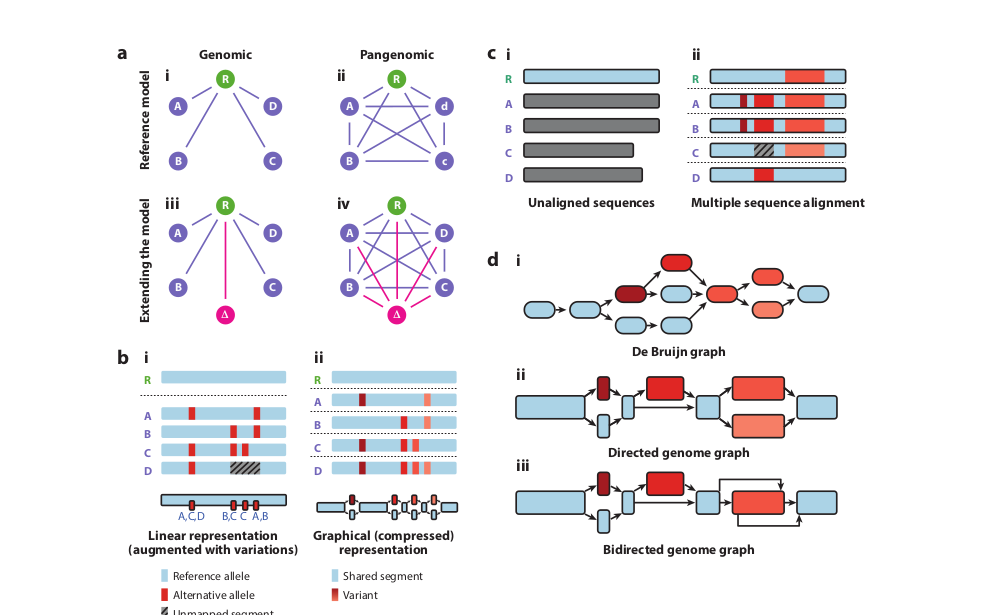
\includegraphics[width=1.00\textwidth]{fig/pangenome_genome.png}
\decoRule
\caption{Genomics versus pangenome (\textbf{A}), Linear representation with variants and Graphical representation compressed (\textbf{B})  Unaligned sequences and multiple sequence alignment (\textbf{C}), three types of graphs(\textbf{D}) \cite{eizenga2020pangenome}}
\label{fig:genomevspangenome.png}
\end{figure}


\section{Genetic variation in graphs}
%TODO: comment Type of variants by size and ability to detect them
The comparison of the sequence of multiple  genomes allow the identification of regions that present differences, i.e. genomic variants (Fig:\ref{fig:typeOfVariants}).  


\begin{figure}[H]
\centering
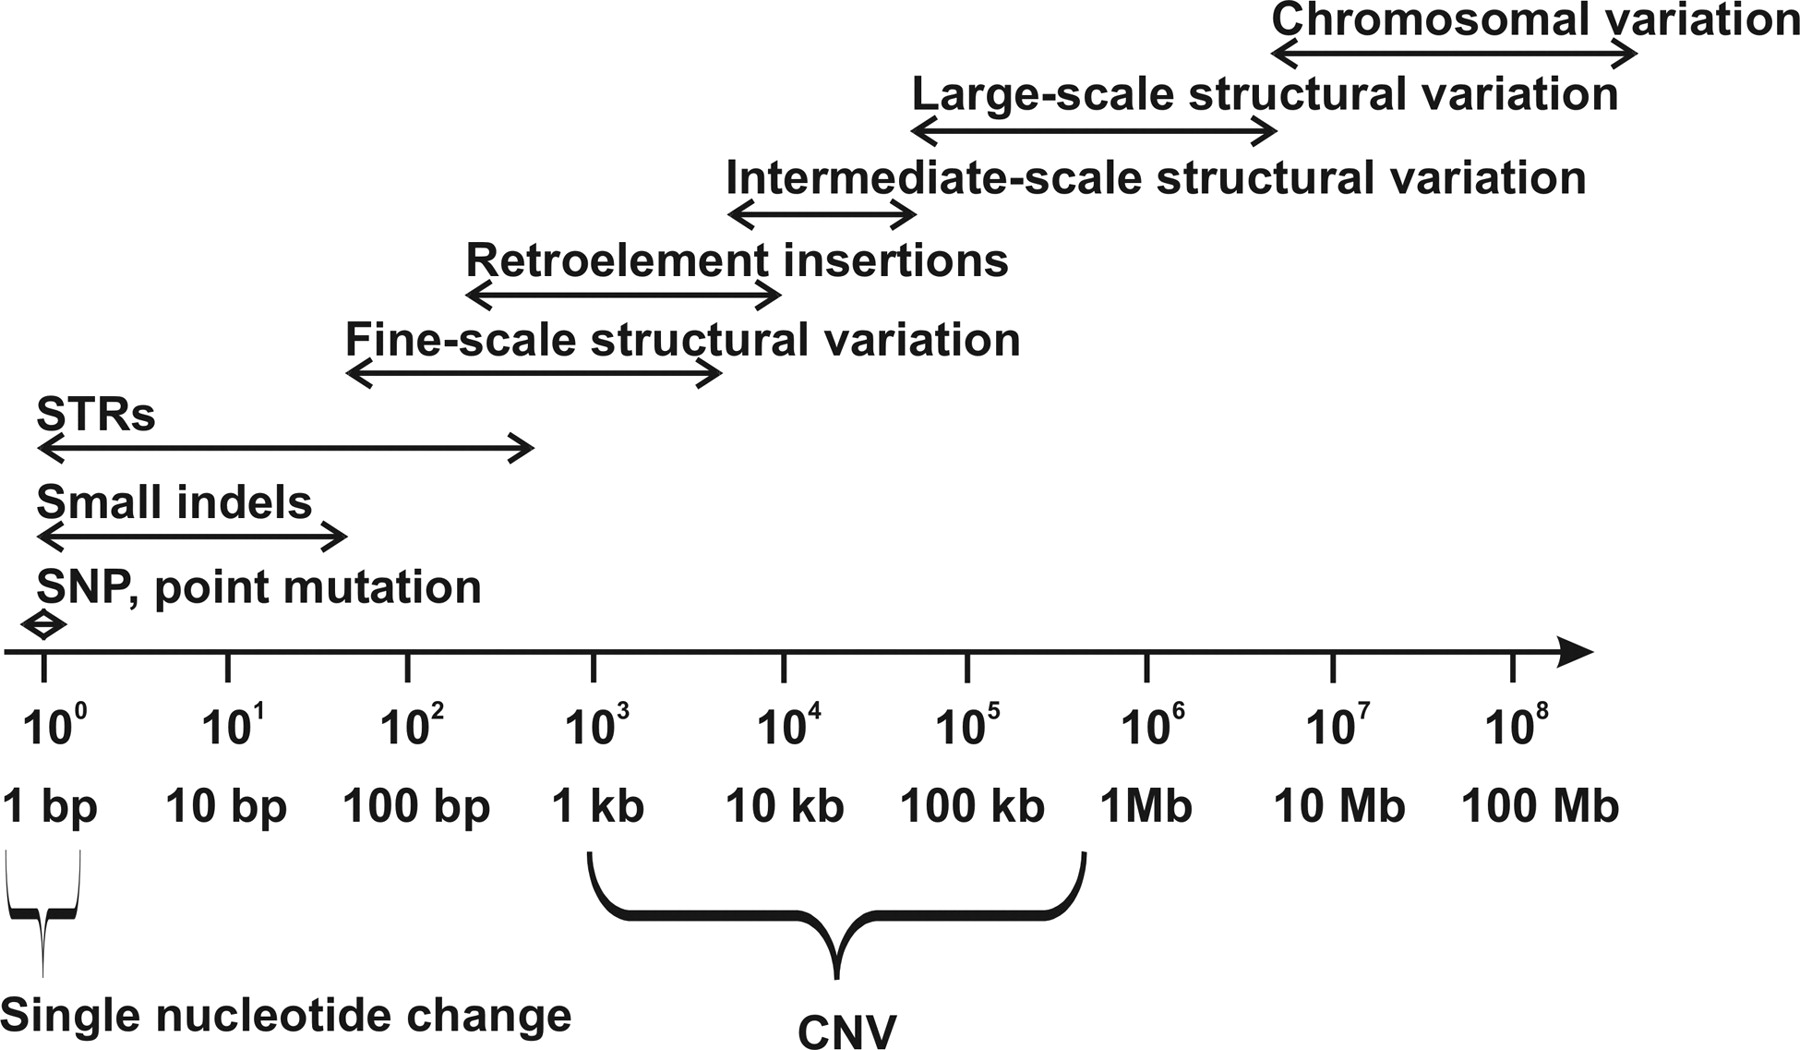
\includegraphics[width=0.7\textwidth]{fig/typeOfVariants.jpeg}
\decoRule
\caption{\textbf{Type and size of genetic variants.}"\textit{Adapted from} \cite{pollex2007copy}"} 
\label{fig:typeOfVariants}
\end{figure}

In graphs genetic variants appear as circles or \textit{bubbles}. In the handlegraph there are five important elements described in Figure \ref{fig:gfa.png}:
\begin{itemize}
\item\textbf{Nodes} represented by yellow rectangles. Each node is associated with a numeric ID and a sequence. 

\item\textbf{Strand Forward and reverse}. DNA strands have forward (+) and reverse (-) orientation. Each node contains a forward and reverse handle (red solid and dashed rectangles, respectively). Handles show the node identifier, the direction (+ or -), and the sequence of the handle.

\item\textbf{Edges} are connections between nodes, repesented by arrows in the figure.

\item\textbf{Paths} are obtained by 'walking' through the graph and represent the actual sequences. Not necessarily all possible paths should be observed in a set of real data.

\item\textbf{Steps} describe paths visits to nodes strands.
\end{itemize}

In (Figure \ref{fig:gfa.png}) the first two paths differ by a single nucleotide polymorphism, with one passing through 2+:T, and the other through 3+:G. The third path is the reverse complement of the first. The fourth is the same as the first, but contains an inversion, passing through 5-: AATC rather than 5+: GATT.



\begin{figure}[H]
\centering
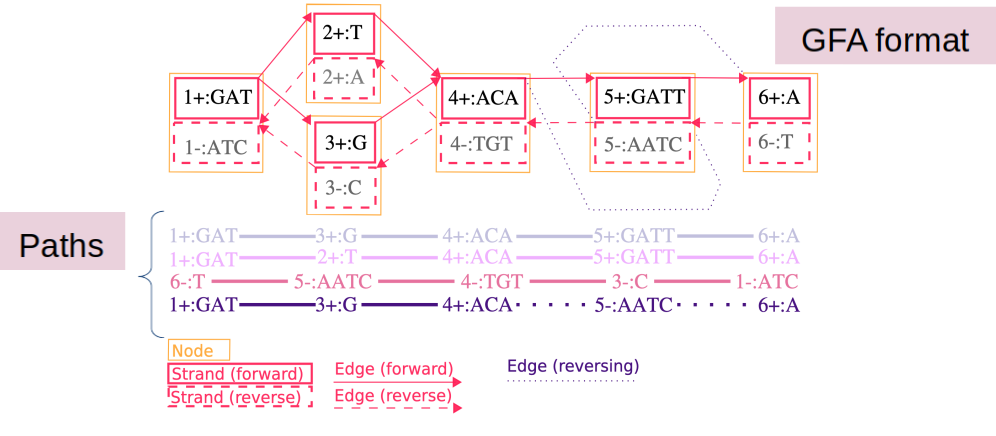
\includegraphics[width=1.00\textwidth]{fig/GFA.png}
\decoRule
\caption{Entities in the bidirected sequence graph (\textbf{A}) \cite{eizenga2020succinct}}
\label{fig:gfa.png}
\end{figure}

When only two variants (of one or more bases) are present, the bubble looks like a circle, while less simple patterns are referred as \textit{superbubbles} (Figure \ref{fig:sup_bub.png})
%Variants are coding in the graph as bubbles. 

\begin{figure}[H]
\centering
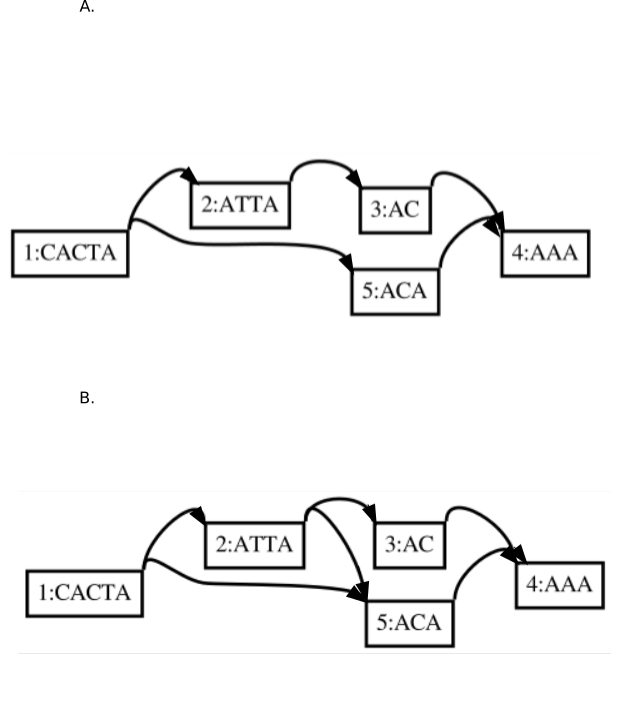
\includegraphics[width=0.50\textwidth]{fig/bub_sup.png}
\decoRule
\caption{Bubble(\textbf{A}), Superbubble (\textbf{B})}
\label{fig:sup_bub.png}
\end{figure}


The superbubble is a more complex subgraph type in which a set of (not necessarily disjoint) paths start and end at common source and sink nodes.\cite{paten2018superbubbles}.
Refering the definition from \cite{onodera2013detecting}, any pair of distinct vertices equation in a digraph (Fig: \ref{fig:sup_bub.png}A):
%OK x e y e X se le metti anche sulla figura altrimenti e' diffcile seguire 
\begin{enumerate}
\item reachability: y is reachable from x.

\item matching: The set of vertices, X, reachable from x without passing through y is equal to the set of vertices from which y is reachable without passing through x (passing through here means to enter and then exit a vertex on the path).

\item acyclicity: The subgraph induced by X is acyclic.

\item minimality: No vertex in X other than y forms a pair with x that satisfies the criteria previously defined, and similarly for y.


\end{enumerate}

%I'm concentred for \textit{bubblepop} to a case specific of a superbubble i.e  bubbles (Fig: \ref{fig:sup_bub.png})
In my project I focused on a specific case of a superbubble i.e. a bubble (Fig: \ref{fig:sup_bub.png}) to implement the core function of the library that is named \textit{bubblepop}. 

A bubble consists of multiple directed unipaths from a vertex\textbf{ v} to a vertex \textbf{u} and is commonly caused by a small number of errors in the centre of reads.\cite{brankovic2016linear}. The bubble may be generalized to the idea of a superbubble, which is a directed, acyclic component of a graph with a single head and tail node.\cite{onodera2013detecting}.

A homologous sequence corresponding to the common start
and end nodes in the bubble flanks two or more alternative alleles in the middle.\cite{garrison2019graphical}.Bubbles can nest and contain more complicated internal structures between the paths
through them. 

\section{Coding of genetic information}

When the genomic information is coded with linear model it is stored in files in Variant Call Format(VCF), whereas graphical representation of a pangenome are stored in Graphical Fragment Assembly (GFA). 



\subsection{Variant Call Format}
Variant Call Format (VCF) is a text file format and is a generic format for storing DNA polymorphism data such as SNPs, insertions, deletions and structural variants, together with rich annotations. (\cite{10.1093/bioinformatics/btr330}). 


\begin{figure}[H]
\centering
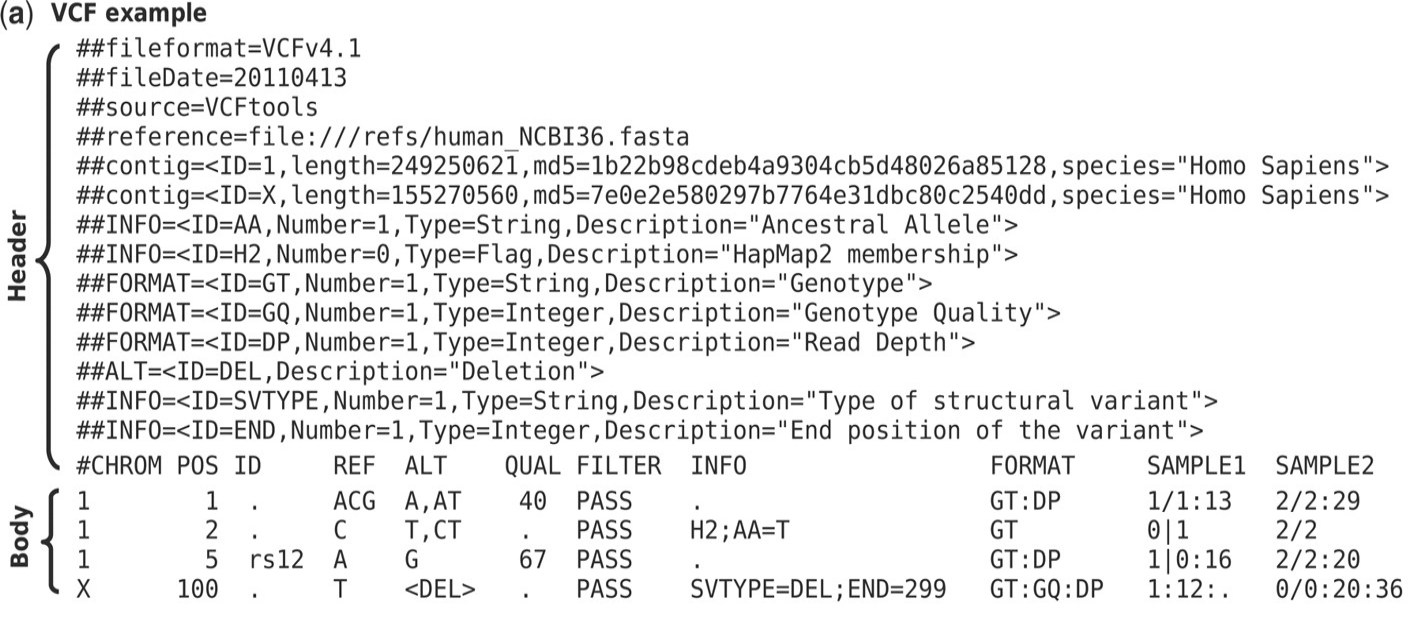
\includegraphics[width=1.00\textwidth]{fig/vcf.png}
\decoRule
\caption{AMPLIARE (\textbf{A}), Linear representation with variants (VCF)) Fig:\cite{10.1093/bioinformatics/btr330}}
\label{fig:vcf.png}
\end{figure}



VCF file (\ref{fig:vcf.png}) consists of:
\begin{itemize}

\item\textbf{Header section}

In the (Fig: \ref{fig:vcf.png}) adapted by (\cite{10.1093/bioinformatics/btr330}) the header contains an arbitrary number of information lines, each starting with characters \#\#, and a TAB delimited field definition line, starting with a single \#,
character. The meta-information header lines provide a standardized description of tags and annotations used in the data section. The use of meta-information allows the information stored within a VCF file to be tailored to the data set in question. It can be also used to provide information about the means of file creation, date of creation, version of the reference sequence, software used and any other information relevant to the history of the file. 

\item\textbf{Data column}

These corresponding to data columns representing the chromosome (CHROM), a 1-based position of the start of the variant (POS), unique identifiers of the variant (ID), the reference allele (REF), a comma separated list of alternate non-reference alleles (ALT), a phred-scaled quality score (QUAL), site filtering information (FILTER) and a semicolon separated list of additional, user extensible annotation (INFO). In addition, if samples are present in the file, the mandatory header columns are followed by a FORMAT column and an arbitrary number of sample IDs that define the samples included in the VCF file. The FORMAT column is used to define the information contained within each subsequent genotype column, which consists of a colon separated list of fields.

\end{itemize}


\subsection{Graphical Fragment Assembly}

Pangenome data are represented by Graphical Fragment Assembly (GFA).(\cite{GFA})

\begin{figure}[H]
\centering
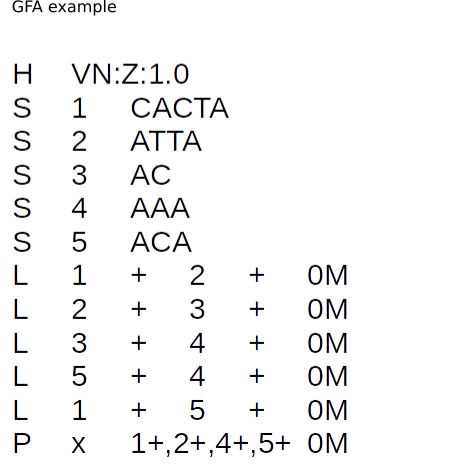
\includegraphics[width=0.50\textwidth]{fig/GFAexample.png}
\decoRule
\caption{Graph representation)} 
\label{fig:GFAexample.png}
\end{figure}

%GFA fatto da me, non copiato, usato per disegnare la bubble della figura precedente 


GFA format is a representation of variation in genomes, splice graphs in genes.





\begin{itemize}

\item\textbf{Header section} start with H.
\item\textbf{Segment line} start with S.
Segment a continuous sequence or subsequence.
\item\textbf{Link lines} start with L.
Link an overlap between two segments. Each link is from the end of one segment to the beginning of another segment. Containment an overlap between two segments where one is contained in the other.
\item\textbf{Path lines} start with P. 
Path an ordered list of oriented segments, where each consecutive pair of oriented segments are supported by a link record.

%dire che ci sono linee opzionali


\end{itemize}

\section{HLA}

\begin{figure}[H]
\centering
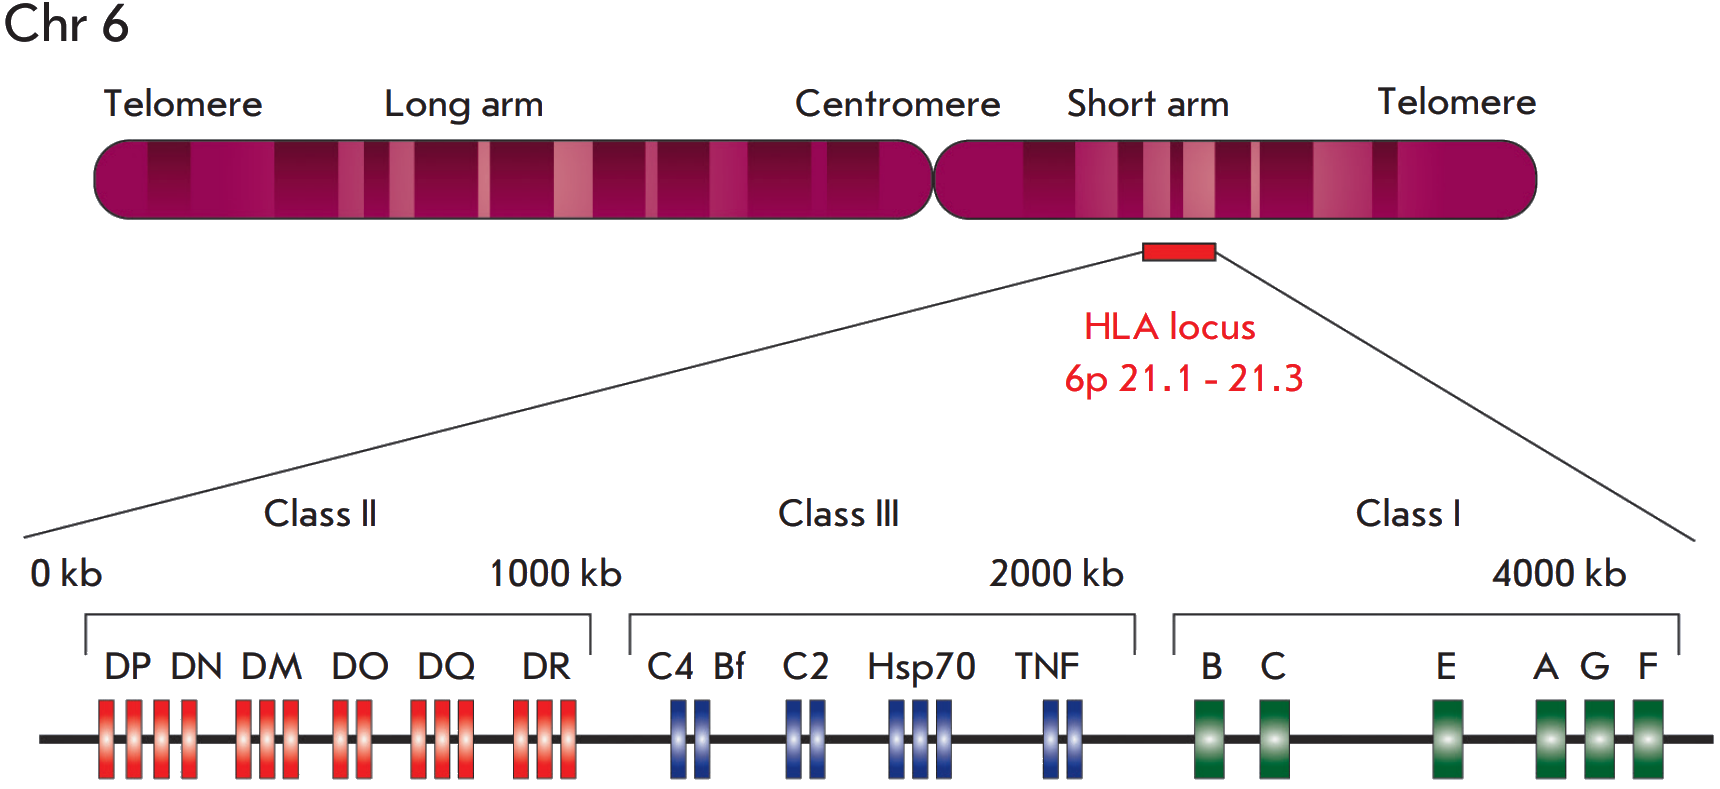
\includegraphics[width=0.80\textwidth]{fig/HLA_loci.png}
\decoRule
\caption{Schematic representation of the HLA locus on human chromosome 6. \cite{zakharova2019contribution})}
\label{fig:HLA.png}
\end{figure}



Genetic studies describes that an important roles in the developing of diseases is played by the major histocompatibility complex (MHC), or human leukocyte antigen (HLA). It contains several gene clusters that encode surface heterodimeric proteins, which are anchored to the plasma membrane and are responsible for antigen presentation to T cells, a stage that is followed by the development of an adaptive immune response. MHC proteins are subdivided into class I, class II, and class III (the complement system) \cite{campbell1993map}.



The HLA region (Fig.\ref{fig:HLA.png}) adapted by \cite{zakharova2019contribution} is located on the short arm of chromosome 6 from 6p21.1 to p21.3 and is shown with a red stripe. The length of class II (red), class III (blue), and class I (green) genes (from the centromeric to the telomeric end) is shown. The class II region includes genes for the $\alpha$ and $\beta$ chains of the MHC class II molecules HLA-DR, HLA-DP and HLA-DQ. In addition, the genes encoding the DMαand DM $\beta$ chains, as well as the genes encoding the $\alpha$ and $\beta$ chains of the DO molecule (DO $\alpha$ and DO $\beta$, respectively), are also located in the MHC class II region.





In the latest version \cite{eggertsson2017graphtyper} of the human reference genome (GRCh38), there are several alternate loci where the sequence variation is too complex to be represented with a single sequence. These loci are generally highly polymorphic, and many are known to co-segregate with disease and are therefore of great interest in population genetics. The most prominent example, the HLA region, is known to associate with a number of human diseases \cite{tiwari2012hla}. 

Short-read sequencing is the standard in genome-wide sequence analysis. Most common approaches for discovering sequence variants involve aligning sequence reads to a reference genome \cite{li2009fast} and searching for variants as alternative sequences in read alignments. However, some reads cannot be aligned to a reference genome, particularly those originating from highly polymorphic regions and regions absent from the reference genome.